Quelle:\\ \href{http://drops.dagstuhl.de/opus/volltexte/2015/4944/pdf/44.pdf}{Visibly Counter Languages and Constant Depth Circuits, Krebs, Lange, Ludwig}
\section{Rückblick}
    Was wir von reg. Sprachen wissen:
    \begin{itemize}
        \item $\Reg$ ist $NC^1$-vollst.
        \item $\Reg\cap AC^0 = FO[Reg.]$
        	= quasi aper. $\gamma:\Sigma^*\to Synt(L)$
        \item $L\in \Reg\setminus AC^0 \Rightarrow L \text{ ist } ACC^0 \text{-schwer}$ (Dichotomie)
        \item $AC^0 \subsetneq ACC_k^0 \subseteq TC^0 \subseteq NC^1 \subseteq L \subseteq NL$\\[1mm]
            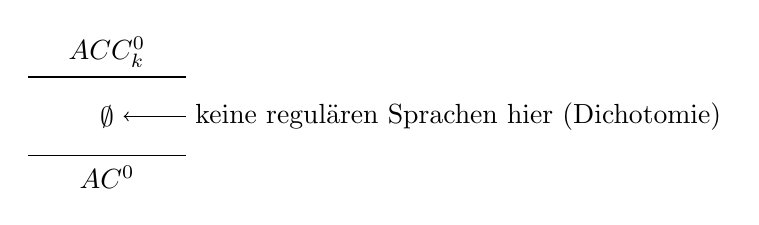
\begin{tikzpicture}
                \draw (0,1) -- (2,1) node[midway, above] (acc) {$ACC_k^0$};
                \node at (1,0.5) (empty) {$\emptyset$};
                \draw [<-] (empty) -- (2,0.5) node [anchor= west] {keine regulären Sprachen hier (Dichotomie)};
                \draw (0,0) -- (2,0) node[midway, below] (ac0) {$AC^0$};
            \end{tikzpicture}
        \item VPL auch $NC^1$-vollständig, also auch $VCL$.
    \end{itemize}
\section{Definition}
    $m-VCA:\ \mathcal{A} = (Q, q_0, E, \Sigma, \delta_0, \dots, \delta_m)$ mit $\delta_i = Q \times \Sigma \to \Sigma$ \\($i$ je nach Ebene, für Ebene $\geq m$ immer $\delta_m$)\\[2mm]
    Akzeptanzkriterium: Endzustand in Lauf erreichbar\\
    $\delta_{min(m, \Delta(w))}$ wird angewandt, nachdem $w$ gelesen wurde. $\Delta(w) = |w|_{call} - |w|_{return}$\\
    \begin{tikzpicture}
        \draw[->] (0,0) -- (0,3);
        \node at (0,1) [anchor=east] (m) {$\delta_m$};
        \draw[dotted] (m) -- (4,1);
        \draw[gray!50] (0,0) -- (1,2) -- (2,1) -- (3,3) -- (4,0);
        \fill[gray!20, pattern=north east lines] (0.5,1) -- (1,2) -- (2,1) -- (3,3) -- (3.667,1) -- cycle;
        \draw[->] (0,0) -- (4,0);
    \end{tikzpicture}
    \subsection{Beispiel}
        \begin{itemize}
            \item $a^nb^n \in 1-VCL$\\
                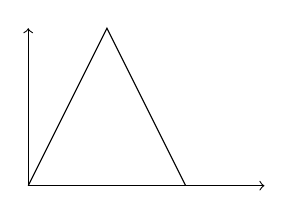
\begin{tikzpicture}
                    \draw[->] (0,0) -- (0,2);
                    \draw[->] (0,0) -- (3,0);
                    \draw (0,0) -- (1,2) -- (2,0);

                    % \draw[->] (4,0) -- (4,2);
                    % \draw[->] (4,0) -- (8,0);
                    % \draw (4,0) -- (4.5,2) -- (5,1) -- (5.5,2) -- (6,1) -- (6.5,2) -- (7,0);
                \end{tikzpicture}
            \item $a^nb^{n-3}a^mb^{m+3} \in 4-VCL$\\
                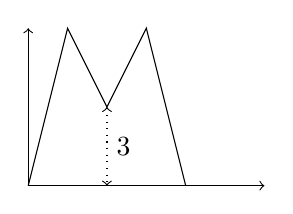
\begin{tikzpicture}
                    \draw[->] (0,0) -- (0,2);
                    \draw[->] (0,0) -- (3,0);
                    \draw (0,0) -- (0.5,2) -- (1,1) -- (1.5,2) -- (2,0);
                    \draw[<->,dotted] (1,1) -- (1,0) node[midway, right] {$3$};
                \end{tikzpicture}
        \end{itemize}
    \subsection{Anmerkung}
        Nicht in $AC^0$:
            \begin{itemize}
                \item $\mathds{D}$, da $TC^0$-schwer
                \item $MAJ,EQU$ (Anzahl $a,b$ vergleichen)
            \end{itemize}
        \subsubsection{Beispiel}
            $L = (a|aba)^nb^n$ ist $TC^0$-schwer
        \subsubsection{Beweis:} zeige $EQU \leq_{AC^0} L$
            \begin{flalign*}
            	f&\in AC^0 \text{ mit } w \in EQU \Leftrightarrow f(w)\in L&\\
            	f(w)&= \varphi(w)\psi(w)\quad \varphi, \psi \text{ Homs.}&\\
            	\varphi(a) &= aaa&\\
            	\varphi(b) &= aba\quad \psi(w)= b^{2|w|}&\\
            \end{flalign*}
            Zu viele $a$'s: 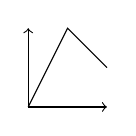
\begin{tikzpicture}\draw[->] (0,0) -- (1,0); \draw[->] (0,0) -- (0,1);\draw (0,0) -- (0.5,1) -- (1,0.5);\end{tikzpicture}$\quad$
            zu viele $b$'s: 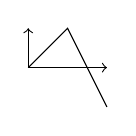
\begin{tikzpicture}\draw[->] (0,0.5) -- (1,0.5); \draw[->] (0,0.5) -- (0,1);\draw (0,0.5) -- (0.5,1) -- (1,0);\end{tikzpicture}
            \begin{flalign*}
            	|w|_a &= |w|_b \rightarrow |f(w)|_a = \frac{3|w|}{2} + \frac{2|w|}{2} = \frac{5}{2}|w|&\\
            	|f(w)|_b &= \frac{|w|}{2} + 2|w| = \frac{5}{2}|w|&\\
            \end{flalign*}
\section{Was macht L schwer?}
    $\rightarrow$ Variable Steigung\\
    Bsp. kann verallgemeinert werden
    \subsection{Definition}
        Zustand q hat \underline{konstante Steigung}, wenn $\exists \alpha \in \mathds{Q}$ ($\alpha$: Steigung) $\forall w \in \Sigma^*$ mit $$ (q,h_1) \xrightarrow{w} (q,h_2)\text{ und}$$
        $\forall w'$ Präfix von $w: h_1 + \Delta(w') \geq m$ gilt:
        $$h_2 = \alpha|w|+h_1 \text{ Steigung}$$
        \begin{tikzpicture}
        	\tikzstyle{dot}=[draw,circle,fill = black, inner sep=0pt,minimum size=2pt]
        	\draw[->] (0,0) -- (5,0);
        	\draw[->] (0,0) -- (0,5);
        	\draw (0,1) -- (-0.1,1) node [left] {$m$};
        	\draw (0,2) -- (-0.1,2) node [left] {$h_1$};
        	\draw (0,4) -- (-0.1,4) node [left] {$h_2$};
        	\node[dot,right] at (1,2) {};
        	\node[dot,right] at (4,4) {};
        	\draw[dashed] (1,2) -- (4,4) node [midway,below] {$\alpha$};
        	\draw plot[smooth] coordinates {(1,2) (1.8,1.6) (2, 3) (2.5, 4) (3,3.5) (3.7, 3.5) (4,4)};
        	\node[left] at (1,2) {$q$};
        	\node[right] at (4,4) {$q$};
        \end{tikzpicture}\\
        Äquivalent (``Korridor''): $$\exists\alpha\in\mathds{Q},\gamma\in\mathds{N}\forall w\in\Sigmas,w'\text{ Präfix von }w:\alpha|w'|-\gamma\le\Delta(w')\le\alpha|w'|+\gamma$$
\section{Einfaches Höhenverhalten}
    \subsection{Definition: aktiver Zustand}
        Zustand $q$ heißt \emph{aktiv}, wenn $\exists w\in L(\mathcal{A})$ und Position $i<j$, sodass $(q_0,0)\overset{w_1\dots w_i}{\longrightarrow}(q,h),h>m+|Q|$ und $h-\Delta(w_1\dots w_j)>|Q|$
    \subsection{Lemma}
        Für $L=L(\mathcal{A})$, sodass $\mathcal{A}$ aktiven Zustand ohne konstante Steigung hat, dann $L\not\in AC^0$ ($TC^0$-schwer)\\
        Beweis: verallgemeinertes Beispiel von oben.
    \subsection{Definition}
        Hat ein VCA $\mathcal{A}$ konstante Steigung in allen aktiven Zuständen, so hat die Sprache $L(\mathcal{A})$ \emph{einfaches Höhenverhalten (EHV)}
    \subsection{Definition: Höhentransduktion}
        $\Tau_m(w):\Sigmas\rightarrow\Sigmas_m, \Sigma_m=\Sigma\times\{0,\dots,m\}$, $\Delta_m(w)=\min(m,\Delta(w))$\\
        $\Tau_m(w)=(w_1,\Delta_m(\epsilon))(w_2,\Delta_m(w_1))(w_3,\Delta_m(w_1w_2))\dots(w_n,\Delta(w_1\dots w_{n-1}))$\\[1mm]
        Beispiel: $\Tau_2(aaba)=(a,0)(a,1)(b,2)(a,1)$\\[1mm]
        $w\in\Sigmas_m$ heißt gültig, wenn $w\in F(\Tau_m(\Sigmas))$ ($F$ Faktor)
    \subsection{Definition}
        gegeben $m$-VCA $\mathcal{A}=(Q,q_0,E,\Sigma,\delta_0,\dots,\delta_m)$ dann $R_\mathcal{A}=L(M)$ mit endlichem Automat $M=(Q,q_0,E,\Sigma_m,\delta)$ mit $\delta(q,(a,i))=\delta_i(q,a)$
    \subsection{Lemma}
        $\mathcal{A}$ ist $m$-VCA, dann $w\in L(\mathcal{A})\Leftrightarrow\Tau_m(w)\in R_\mathcal{A}$\\
        Also: Wortproblem von $L(\mathcal{A})$ zweiteilbar:
        \begin{itemize}
            \item berechne $\Tau_m(w)$
            \item teste ob in $R_\mathcal{A}$
        \end{itemize}
        Bisher: $\neg EHV\Rightarrow\not\in AC^0$ (da $\Tau_m\not\in AC^0$)\\
        Jetzt: $EHV\Rightarrow \Tau_m\in AC^0$ berechenbar
    \subsection{Satz}
        EHV$\Rightarrow$ Höhenprädikat $H_m(x)$ in $FO[+]$ definierbar
        \begin{itemize}
            \item $w_{x=i}\models H_k(x)\Rightarrow\Delta(w_1\dots w_{i-1})=k$ falls $w\in\Sigmas$
            \item $w_{x=i}\models H_k(x)\Leftrightarrow\Delta(w_1\dots w_{i-1})=k$ falls $w\in L$
        \end{itemize}
        \subsubsection{Beweisidee}
            EHV $\overset{1.}{\rightarrow}$ Matching-Prädikat $\overset{2.}{\rightarrow}$ Höhenprädikat
            \begin{enumerate}
                \item $M(x,y)$ ist wahr, wenn well-matched zwischen $x$ und $y$\\
                    Betrachte Fall große Höhe und aktive Zustände:\\
                    \begin{itemize}
                        \item Fasse Schleifen zusammen:\\
                            Bsp.: $q_1\underbrace{q_2q_3q_2q_4q_2}_{q_2}q_5q_6\leadsto q_1q_2q_5q_6$
                            (jeder Zustand höchstens $1\times\Rightarrow$ endliche Kombinationsmöglichkeiten $|Q|!$ für komprimierte Läufe)
                        \item Jeder Zustand deckt Bereich mit konstanter Steigung ab $\Rightarrow$ Wort ist aufteilbar in höchstens $|Q|!$ Abschnitte konstanter Steigung
                        \item Formel für $M(x,y)$: rate Lauf und verifiziere Steigungen ($n=|Q|$):\\
                        $M(x,y)=x<y\wedge\Sigmapush(x)\wedge\Sigmapop(y)\wedge\\
                        \bigvee\limits_{(q_1,\dots,q_n)\in Q^n}
                        \left(\vphantom{\bigwedge\limits_{i=0}^{n-1}} %vertical space only
                        \exists z_0,\dots,z_n\exists h_0,\dots,h_n: z_0=x\wedge z_n=y-1\wedge h_0=h_n\wedge\right.\\
                        \left.\bigwedge\limits_{i=0}^{n-1}z_i\le z_{i+1}\wedge A_{q_{i+1}}(z_i,z_{i+1},h_i,h_{i+1},h_0)\right)$ (Definition von $A_{q_{i+1}}$: Paper)
                    \end{itemize}
            \end{enumerate}
\section{Der reguläre Anteil einer VCL}
    $\exists \mathcal{A}:R_\mathcal{A}\in AC^0\Rightarrow \exists FO[reg]$-Formel\\
    $\forall\mathcal{A}:R_\mathcal{A}\not\in AC^0\Rightarrow L(\mathcal{A})\not\in AC^0$
    \subsection{Beispiel}
        $L=\{wb^{|w|}\mid w\in\{a_1,a_2\},|w|_{a_1}\equiv 0\pmod 2\}$\\
        $\mathcal{A}$ mit $L(\mathcal{A})=L$, dann ``$R_\mathcal{A}=Parity(a_1,a_2)b^*$''\\
        $L'=L\cap\Sigma^{10}\in AC^0$ $(L(R_{\mathcal{A}'})=L')$\\
        aber $R_{\mathcal{A}'}$ könnte:
        \begin{itemize}
            \item endlich sein $\Rightarrow R_{\mathcal{A}'}\in AC^0$
            \item ``$R_{\mathcal{A}'}=Parity(a_1,a_2)b^{10}$''$\Rightarrow R_{\mathcal{A}'}\not\in AC^0$
        \end{itemize}
        $\Rightarrow$ Lösung: Normalform\\
        Problem: Schleife, die $R_\mathcal{A}$ komplex macht aber unnötig ist.
    \subsection{Definition (informell)}
        $\mathcal{A}$ heißt Schleifen-normal, wenn jede Schleife synchron pumpbar ist.
    \subsection{Lemma}
        Für jeden VCA $\mathcal {A}$ existiert Schleifen-normaler Automat $\mathcal{A}'$ mit $L(\mathcal{A})=L(\mathcal{A}')$
    \subsection{Lemma}
        Ist $\mathcal{A}$ Schleifen-normaler $m$-VCA, dann:\\
        $\exists t>0\ \exists G\subseteq\Sigma^t_m$ mit $G^*\subseteq F(\Tau_m(\Sigmas))$, sodass $\eta_{R_\mathcal{A}}(G)$ nicht-triviale Gruppe enthält, dann $L(\mathcal{A})\not\in AC^0$ (vgl. quasi-aperiodisch)
    \subsection{Satz (Wdh.)}
        Ist $L$ regulär, dann $L\in AC^0\Leftrightarrow\forall t>0\forall G\subseteq\Sigma^t:\eta_L(G)$ hat nur triviale Gruppen $\Leftrightarrow L\in FO[reg]$
    \subsection{Lemma}
        $\forall t>0\forall G\subseteq\Sigma_m^t$ mit $G^*\subseteq F(\Tau_m(\Sigmas))$, so dass $\eta_{R_\mathcal{A}}$ hat nur triviale Teilgruppen $\Rightarrow\exists FO[reg]$-Formel $\varphi$ mit $L(\varphi)\cap\Tau_m(\Sigmas)=R_\mathcal{A}\cap\Tau_m(\Sigmas)$
    \subsection{Satz}
        Sei $\mathcal{A}$ ein Schleifen-normaler $m$-VCA für $L=L(\mathcal{A})$.\\
        $L\in AC^0\Leftrightarrow L$ hat EHV und $\forall t>0\forall G\subseteq\Sigma_m^t$ mit $G^*\subseteq F(\Tau_m(\Sigmas))$ hat $\eta_{R_\mathcal{A}}$ nur triviale Teilgruppen.
        \subsubsection{Beweis}
            Beginne mit $FO[reg]$-Formel $\varphi$ mit $\underbrace{L(\varphi)}_{\subseteq\Sigmas_m}\cap\Tau_m(\Sigmas)=R_\mathcal{A}\cap\Tau_m(\Sigmas)$.\\
            $Q_{(a,i)}x$-Prädikate in $\varphi$ ersetzen durch
            \begin{itemize}
                \item $(Q_ax\wedge H_ix)$, falls $i<m$
                \item $(Q_ax\wedge H_{\geq m}x)$, falls $i\geq m$
            \end{itemize}\qed\\
            Alternative Sichtweise: $\Tau_m^{-1}(L(\varphi))=\Tau_m^{-1}(R_\mathcal{A})$\\
            %als Schaltkreis...
    \subsection{Satz}
        Gegeben $\mathcal{A}$, dann ist es entscheidbar, ob $L(\mathcal{A})\in AC^0$
        \subsubsection{Beweis}
            Betrachte Schleifen-normalen Automaten $\mathcal{A}'$
            \begin{itemize}
                \item Überprüfe EHV: $\forall q\in Q:$ ``$q$ aktiv $\Rightarrow$ konstante Steigung''
                \begin{itemize}
                    \item konstante Steigung: teste $w\in\Sigma^{\le|Q|}$, die durch $q$ schleifen. Haben alle die gleiche Steigung?
                    \item aktiv: finde $x$ mit $\Delta(x)>m+|Q|$ und $y$ mit $xy\in L(\mathcal{A})$ mit $y=y'y''$ mit $\Delta(y')>-|Q|$
                    \begin{itemize}
                        \item ``$x$ finden'' auf Leerheitsproblem für VCL reduzierbar
                        \item $y:\Delta(x)\cdot|Q|$ maximale Länge
                    \end{itemize}
                \end{itemize}
                \item regulärer Anteil: analog quasi-aperiodisch für reguläre Sprachen.\qed
            \end{itemize}
\section{Anmekung}
    $VPL\cap AC^0$ noch offen
    \subsection{Beispiel}
        \begin{itemize}
            \item $S\rightarrow a_1Sb|a_2Sbc|\epsilon$
            \item $S\rightarrow aSbc|acSb|\epsilon$\\
                 unbekannt ob $\in AC^0$
        \end{itemize}
        vgl. $S\rightarrow aSb|aSbc|\epsilon$ ($\in VCL,\ \not\in AC^0$)
